\section{Rényi's $\alpha$-Divergence and Kullback-Leibler Divergence}

\begin{figure}[H]
    \centering

    \textbf{Unknown Variance}
    
    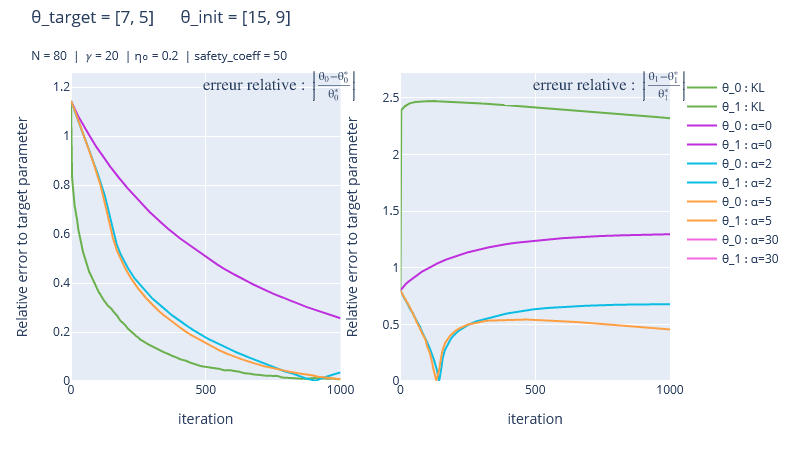
\includegraphics[height=0.32\pdfpageheight]{Images/simulation/normal_case/KL_and_Renyi_unkown_variance.png}

    \textbf{Known Variance}
    
    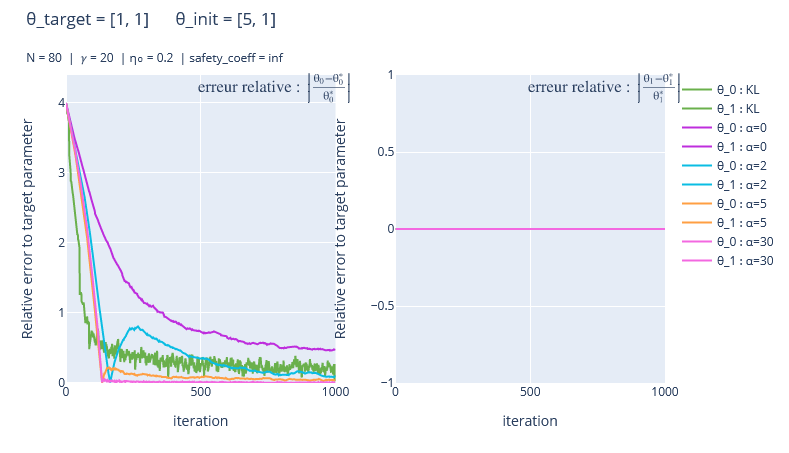
\includegraphics[height=0.32\pdfpageheight]{Images/simulation/normal_case/KL_and_Renyi_kown_variance.png}

    
    \begin{align*}
    \widehat{\nabla R_\alpha}(t) = \displaystyle{ \alpha  \sum\limits_{i=1}^N  \left[\frac{\left( \frac{f(x_i)}{q_t(x_i)} \right)^{1-\alpha}}{\sum\limits_k \left(\frac{f(x_i)}{q_t(x_i)}\right)^{1-\alpha}}\right] \cdot \frac{\widehat{\nabla_\theta} {q_t}(x_i)}{q_t(x_i)}} 
    & \, &
    \widehat{\nabla_\theta L}(\theta_t) = \displaystyle\sum\limits_{i=1}^{N} \underbracket{\displaystyle\frac{f(x_i)}{q_{\theta_t}(x_i)}}_{\omega_t(X_i)} \nabla_\theta \left[ h_{\theta_t}(x_i)\right] \\
    & \, &
    \end{align*}
    
    
    \caption{Simulations of SGA using normal distribution for $f$ and $q_{\theta_t}$: comparing Rényi and Kullback-Leibler Divergence}
    \label{sim:KL-and-R}
\end{figure}

\begin{figure}[H]
    \centering
    \label{sim:renyi-other-distrib}
    \begin{minipage}{0.5\textwidth}
    \centering
    \textbf{Exponential}
    
    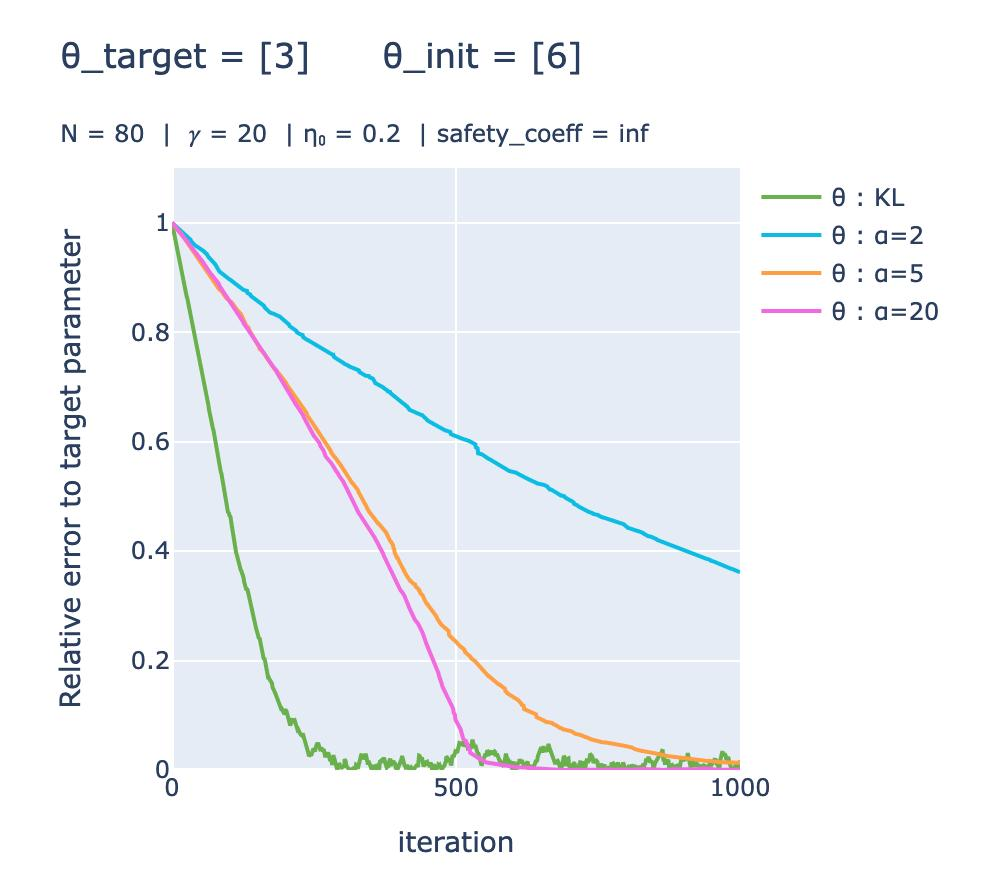
\includegraphics[width = \linewidth]{Images/simulation/exponential_renyi.jpeg}
    \end{minipage}
    \begin{minipage}{0.48\textwidth}
    \centering
    \textbf{Student}
    
    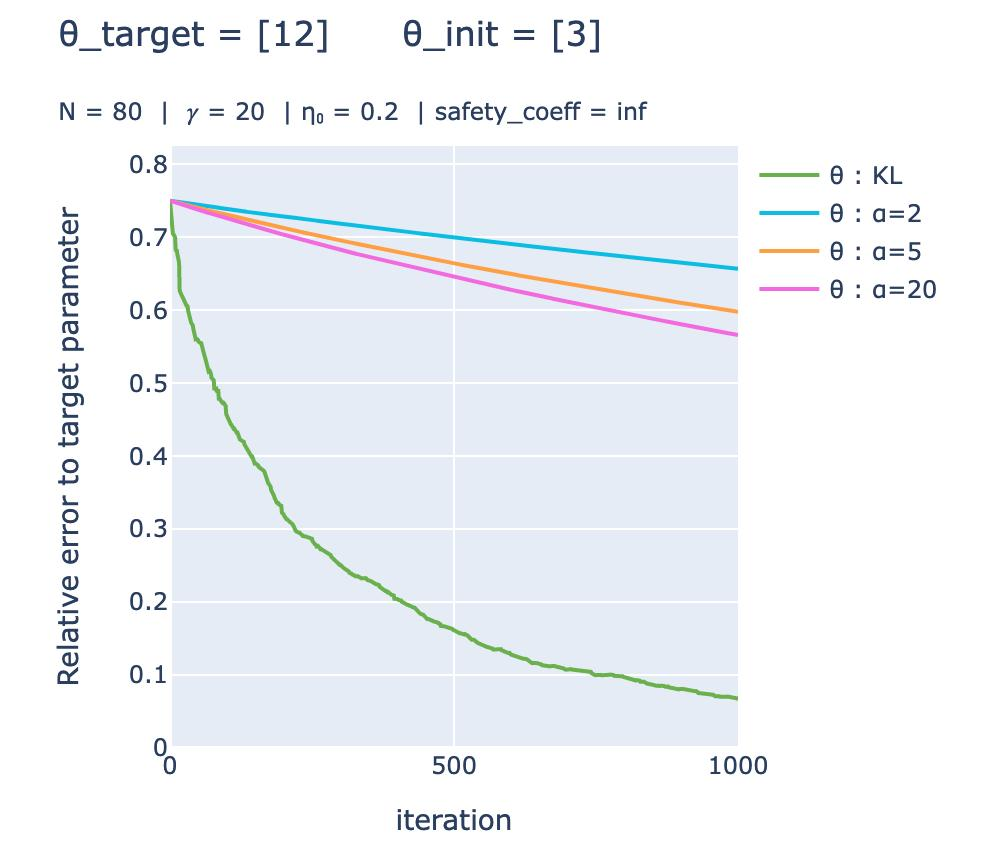
\includegraphics[width = \linewidth]{Images/simulation/student_renyi.jpeg}
    
    \end{minipage}
    \caption{Rényi's divergence criterion for Stochastic Gradient Descent using other distribution families}
\end{figure}

\pagebreak

\section{wAIS Simulations}

Figure 7 depicts the distribution of wAIS estimates, once for the Kullback-Leibler criterion (upper panel) and once for Rényi's alpha divergence with $\alpha = 2$ (lower panel). For every scenario, the distribution is made up of a total of 30 estimates:
\begin{itemize}

    \item T = 5
    \begin{itemize}
         \item 30 estimations of $\mu$ with update frequency: every iteration (blue)
         \item 30 estimations of $\mu$ with update frequency: every two iterations (red)
    \end{itemize}
    \item T = 20 and T = 50
        \begin{itemize}
         \item 30 estimations of $\mu$ using an update frequency: every four iterations (red)
         \item 30 estimations of $\mu$ using update frequency: every two iterations (green)
    \end{itemize}
    % \item T = 50
    %     \begin{itemize}
    %      \item 30 estimations of $\mu$ using an update frequency: every four iterations (red)
    %      \item 30 estimations of $\mu$ using update frequency: every two iterations (green)
    % \end{itemize}
\end{itemize}


\begin{figure}[H]
    \centering
    \label{sim:wais-KL-and-R}
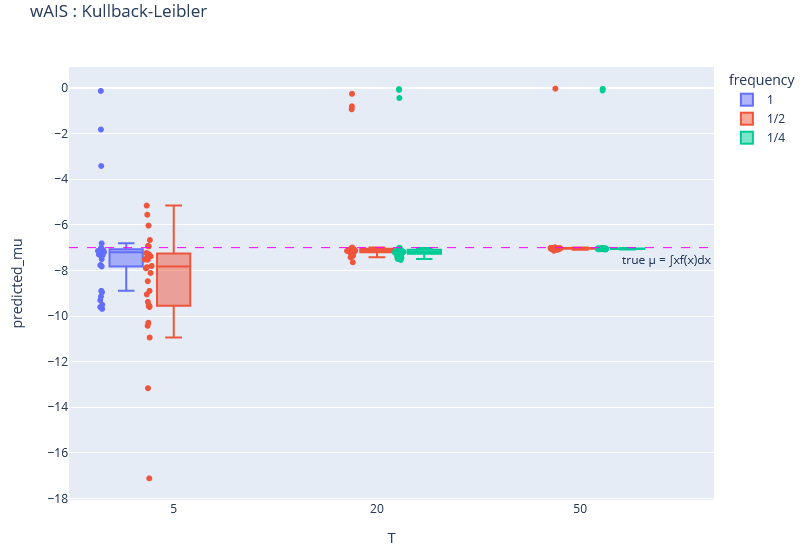
\includegraphics[height=0.30\pdfpageheight]{/simulation/wais/wais_KL_all.png}

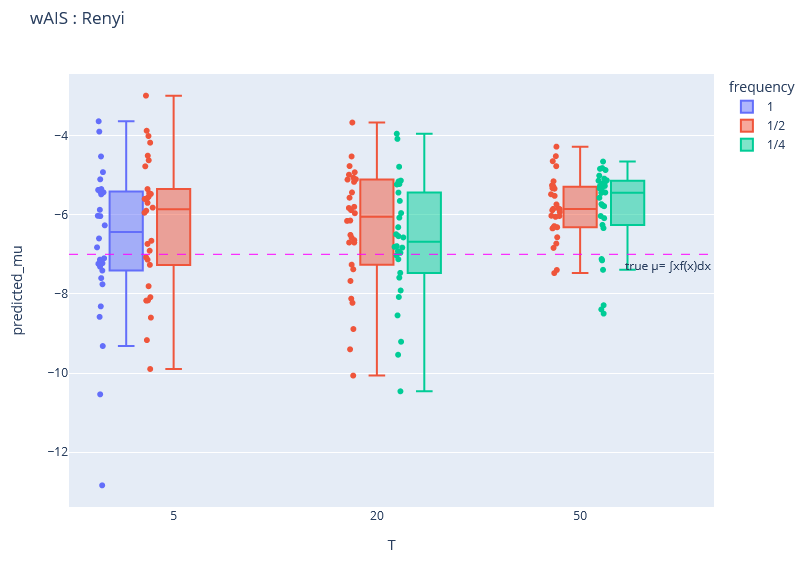
\includegraphics[height=0.30\pdfpageheight]{/simulation/wais/wais_renyi_all.png}
    \caption{Distribution of the estimates of $\mu_*$ = -7 from a normal distribution using wAIS}
    
\end{figure}

